\chapter{Fondamenti}

\section{Intrusion Detection System}


Un intrusione può essere definita come un evento che compromette integrità, confidenzialità e la disponibilità di un sistema informatico \cite{biermannComparisonIntrusionDetection2001}.

Gli Intrusion Detection System (IDS) sono delle soluzioni hardware o software che, posti all'interno di una rete o di un sistema, rilevano eventuali intrusioni. 

Questi strumenti sono essenziali per tenere al sicuro le persone da attacchi informatici ~\cite{SurveyIntrusionDetection2019}.

\cite{ashoorImportanceIntrusionDetection2010} Le principali funzioni degli IDS sono: 

\begin{itemize}
    \item Monitorare ed analizzare sia le attività utente che di sistema
    \item Tracciare le violazioni delle policy utente
    \item Analizzare le configurazioni e le vulnerabilità del sistema
    \item Rilevare tipici attacchi di rete
    \item Analizzare attività anomale
\end{itemize}


\cite{liaoIntrusionDetectionSystem2013} Solitamente gli IDS vengono classificati in base al tipo di analisi che effettuano e come questi rilevano le minacce. Ne esistono di tre tipi principali:


\begin{itemize}
    \item Signature-Based Detection (SD)
    \item Anomaly-based Detection (AD)
    \item Stateful Protocol Analysis (SPA)
\end{itemize}



\subsection{Signature-Based Detection}

Questo tipo di rilevamento utilizza la firma di un attacco per poterlo rilevare. Quindi conoscendo questa firma, gli IDS la comparano agli eventi catturati della rete. Dato che questi attacchi hanno bisogno di una conoscenza pregressa sono anche chiamati Knowledge-based.


\subsection{Anomaly-based Detection}

Gli Anomaly-based Intrusion Detection Systems (AIDS) sono stati introdotti per sopperire alle mancanze del Signature-Based Detection.
Questo tipo di rilevamento utilizza un modello che rappresenta il normale comportamento della rete. Se viene rilevato un evento che non è coerente con il modello di riferimento, allora viene segnalata un'anomalia. Questo tipo di rilevamento è chiamato anche Behavior-Based.


Il principale vantaggio di questo tipo di IDS è la possibilità di rilevare gli attacchi zero-day \cite{UnsupervisedAlgorithmsDetect2021}, in quanto questi sistemi, non si basano sulla firma dei dati o su regole rigide. Tra gli altri vantaggi si ha che risulta essere difficile, per un eventuale criminale, capire quale sia il comportamento normale di un utente senza produrre un segnale da parte del sistema \cite{SurveyIntrusionDetection2019}.


Gli AIDS possono essere classificati in base al metodo utilizzato per la loro implementazione:

\begin{itemize}
    \item Basati sulla Statistica (Statistical-Based)
    \item Basati sulla Conoscenza (Knowledge-Based)
    \item Basati sull'apprendimento automatico (Machine Learning-Based)
\end{itemize}


Gli AIDS Statistical-Based dopo aver registrato i dati di una porzione di elementi, derivano il modello statistico di un utente nella rete. 


I Knowledge-based invece, utilizzano regole predefinite per generare il modello di riferimento.
Dall'altra parte troviamo gli AIDS Machine Learning-Based, che utilizzano un algoritmo di apprendimento automatico per generare il modello di riferimento. 

La figura ~\ref{fig:aids_classification} mostra più in dettaglio questo tipo di classificazione e i metodi di implementazione associati.

\begin{figure}[htpb]
    \centering
    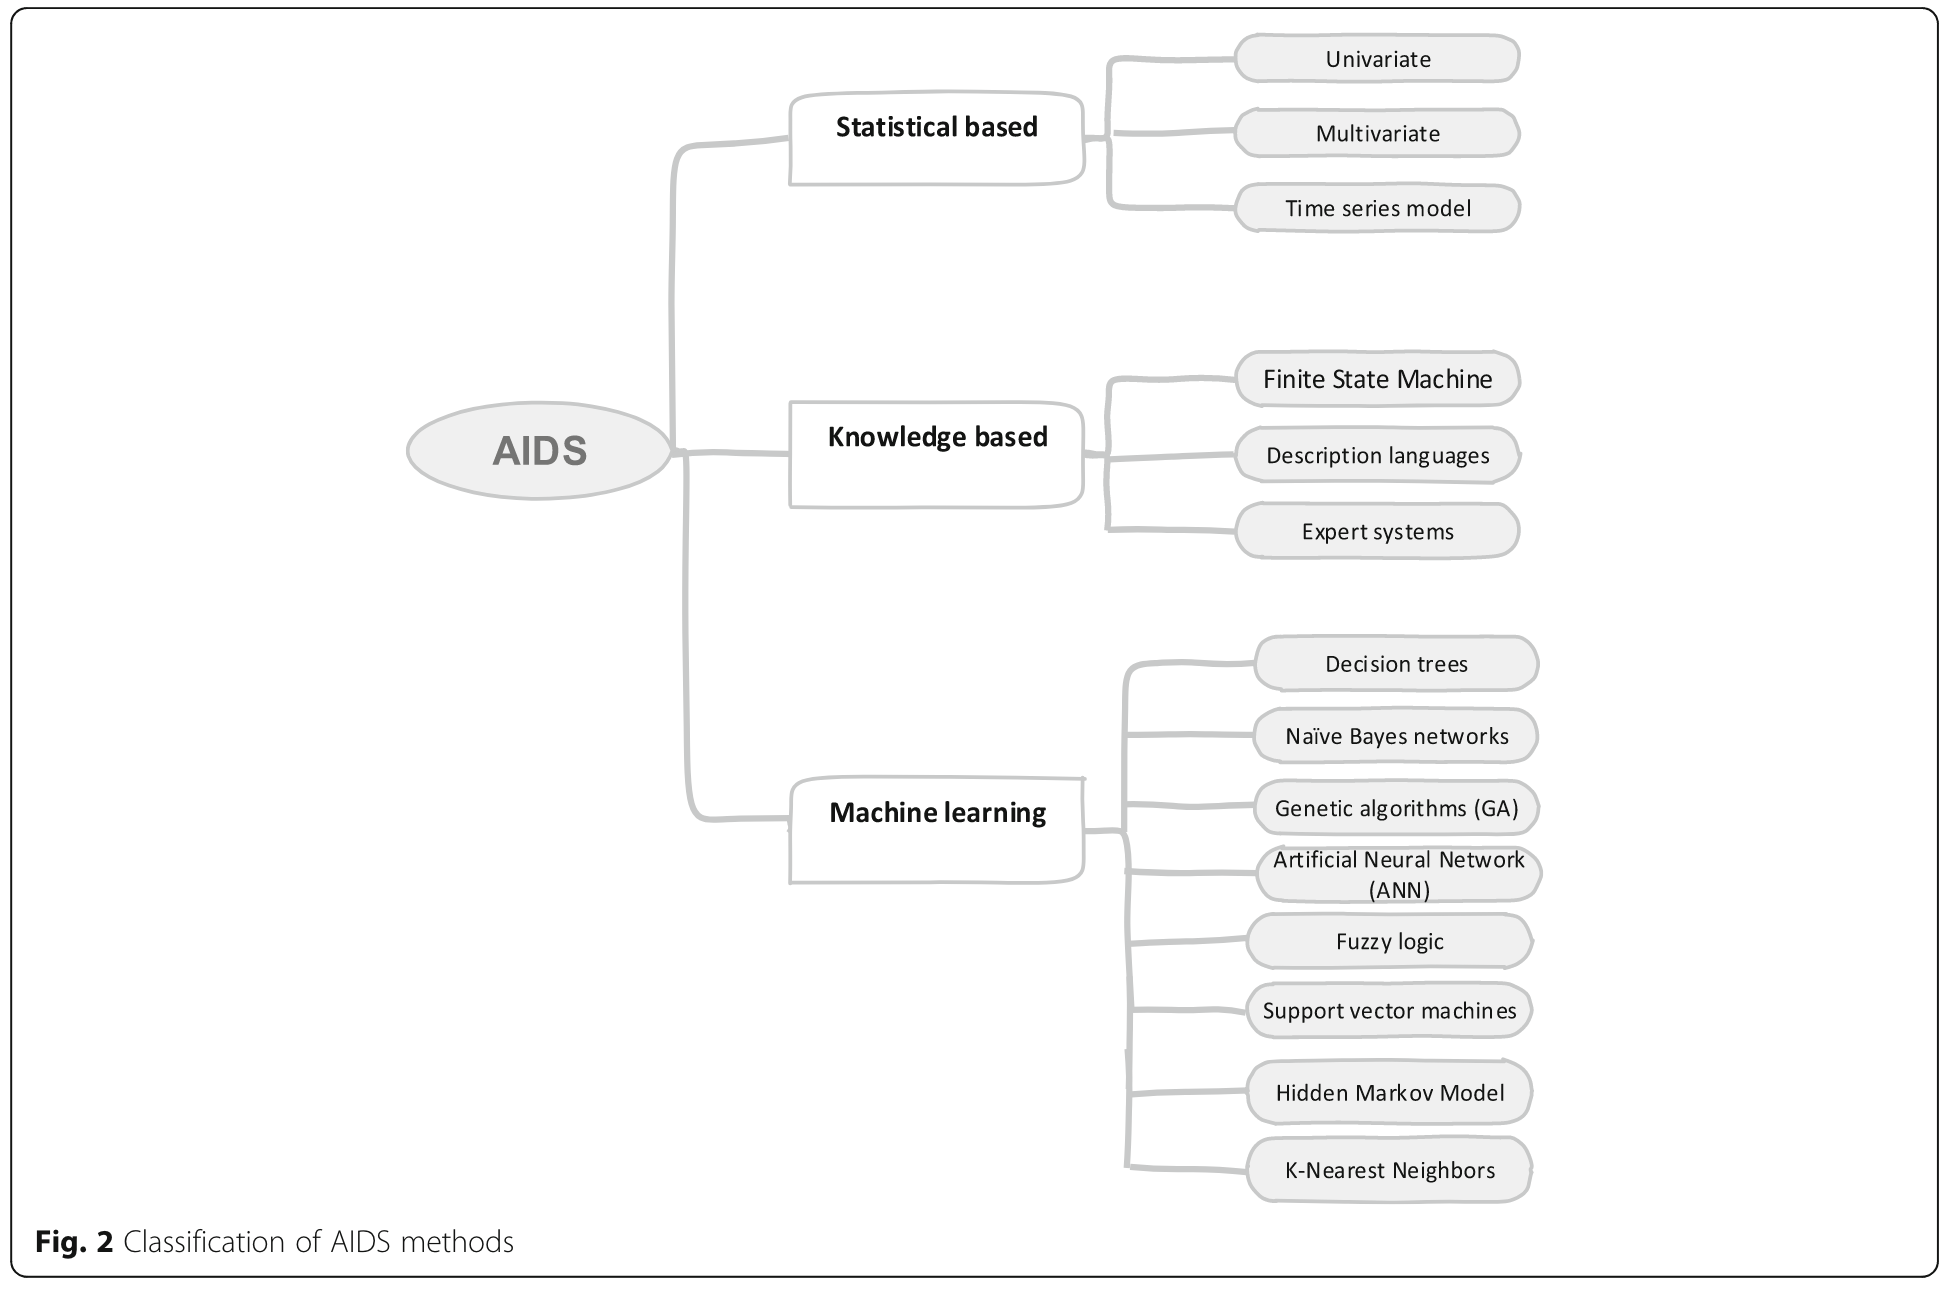
\includegraphics[width=\textwidth,height=10cm,keepaspectratio=true]{img/aids_classification.png}
    \caption{
        Schema che riassume i vari metodi di implementazione degli AIDS, da \cite{SurveyIntrusionDetection2019}. I modelli sono divisi nelle tre categorie descritte precedentemente, ma sono presenti anche i vari tipi di algoritmi utilizzati.
    }
    \label{fig:aids_classification}
\end{figure}


\subsection{Stateful-Protocol-Analysis}

In questo caso gli IDS conoscono lo stato e le specifiche del protocollo utilizzato. Vengono quindi rilevati degli eventi che non rispettano gli standard del protocollo, generalmente quelli da specifica e.g. IEEE.

Potrebbe sembrare che gli AD e gli SPA siano simili, in realtà i primi, conoscono il comportamento di una specifica rete,  mentre i secondi, conoscono solo gli standard dei protocolli.



\section{Machine Learning per rilevamento di intrusioni}


Il Machine Learning (ML) è un sottoinsieme dell'intelligenza artificiale e permette ai sistemi di imparare dai dati e di migliorare le loro prestazioni nel tempo senza essere esplicitamente programmati. Nel caso degli Intrusion Detection Systems, gli algoritmi di ML permettono di rilevare in maniera precisa e rapida gli attacchi per grandi quantità di dati in poco tempo ~\cite{saranyaPerformanceAnalysisMachine2020}.


Solitamente questi algoritmi sono divisi in:

\begin{itemize}
    \item Supervised
    \item Unsupervised 
\end{itemize}

Inoltre gli algoritmi di ML possono essere usati per la classificazione o per la predizione.

Il processo di classificazione si compone di vari passi tra cui:

\begin{itemize}
    \item Preprocessamento dei dati
    \item Definizione dei dati di test
    \item Scelta dell'algoritmo
    \item Impostazione dei parametri
    \item Addestramento del modello
    \item Test del modello
\end{itemize}

come mostrato in figura \ref{fig:ml_process}.

\begin{figure}[htpb]
    \centering
    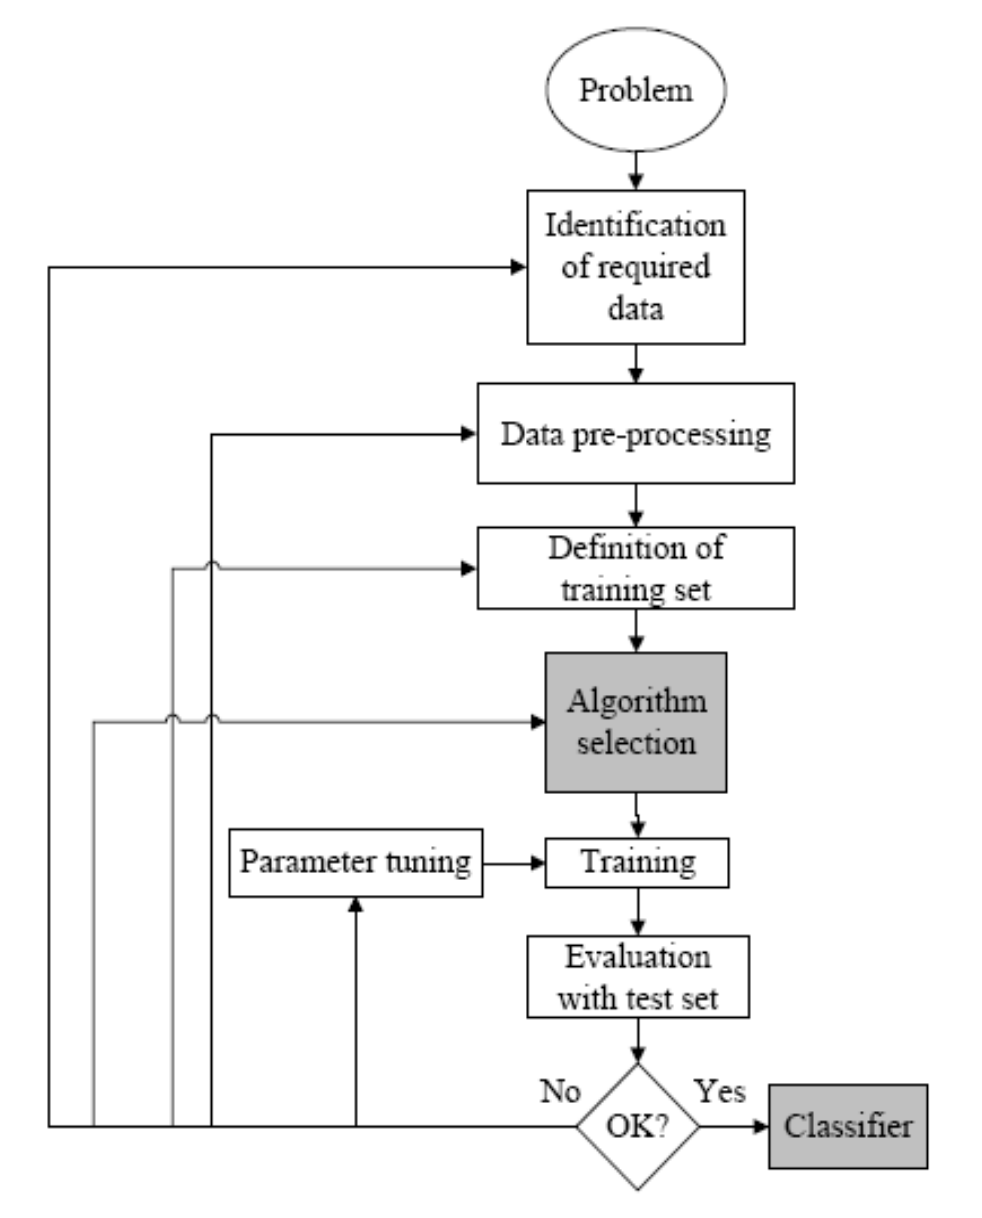
\includegraphics[width=\textwidth,height=10cm,keepaspectratio=true]{img/ml_process.png}
    \caption{
        Il processo del Supervised Machine Learning, da \cite{babcockuniversitySupervisedMachineLearning2017}
    }
    \label{fig:ml_process}
\end{figure}


Il modello viene addestrato su un dataset con classi conosciute e cerca di trovare una relazione tra le caratteristiche dei dati (features) e le classi stesse. 
In particolare un classificatore mappa una funzione: 

\[
  f(x_1,\ldots x_S) \leftrightarrow \overline{y}
\]

che assegna uno scalare facente parte di un insieme $C$ di elementi disgiunti (le classi), ad un insieme di $S$ elementi vettoriali (le caratteristiche) ~\cite{hoffmannBenchmarkingClassificationRegression2019}.


Nella regressione invece, si cerca di approssimare la funzione: 

\[
f(x_1,\ldots x_S) \leftrightarrow y
\]

a partire dalle caratteristiche. La funzione $f$ è approssimata utilizzando varie tecniche di interpolazione, estrapolazione, analisi di regressione e curve fitting ~\cite{hoffmannBenchmarkingClassificationRegression2019}.


Nel nostro caso utilizzeremo un algoritmo di classificazione.




\subsubsection{Supervised Machine Learning}

Il Supervised Machine Learning utilizza un dataset con classi completamente etichettate cercando di trovare una relazione tra gli elementi del dataset e le classi di questi dati. 
I dataset utilizzati per l'addestramento, necessitano di essere catalogati precedentemente.
Ci sono vari algoritmi di questo tipo e.g. Support Vector Machine (SVM), Naïve Bayes, Reti Neurali, Alberi di Decisione, Random Forest.


\subsubsection{Unsupervised Machine Learning}

In questo caso, gli algoritmi di ML non hanno un dataset con classi etichettate. Questi algoritmi trovano delle relazioni tra i dati, cercando di raggrupparli in base a delle caratteristiche comuni.

L'unsupervised machine learning mostra però basse prestazioni per quanto riguarda il rilevamento quindi non possono essere utilizzati come principale strumento per gli IDS. Il motivo di questo scarso rendimento è dovuto al fatto che è molto probabile generare dei Falsi Positivi (vengono rilevati attacchi quando in realtà non cene sono) oppure generare dei Falsi Negativi (non vengono rilevati attacchi quando in realtà ce ne sono) questo va a degradare le performance generali del modello.

D'altra parte però questi modelli si sono dimostrati opinabilmente migliori per rilevare gli attacchi zero-day. ~\cite{UnsupervisedAlgorithmsDetect2021}.


\section{XGboost}

XGBoost (eXtreme Gradient Boosting) è un algoritmo di Machine Learning che utilizza alberi di decisione per la classificazione e la regressione. 

Nel mondo reale è utilizzato anche per la predizione dei click per le pubblicità  ~\cite{hePracticalLessonsPredicting2014} e come algoritmo per le competizioni su Kaggle ~\cite{chenXGBoostScalableTree2016}.


Il suo punto di forza principale è la grande scalabilità in tutti gli scenari. XGBoost ha prestazioni superiori di dieci volte rispetto alle soluzioni esistenti.
Inoltre riesce a sfruttare al meglio la potenza di calcolo della macchina su cui viene eseguito ~\cite{chenXGBoostScalableTree2016}.
È stato scelto questo modello per i motivi sopra citati.

\subsection{Alberi di Decisione}

Nella sua parte fondamentale XGBoost utilizza gli alberi di decisione.

Un albero di decisione è uno strumento relativamente semplice per classificare i dati dove vengono poste delle domande che riguardano le features. Ogni domanda è contenuta in un nodo dell'albero, ed ognuno di questi punta ad un figlio che rappresenta una possibile risposta.
In questo modo le domande formano una gerarchia (Figura \ref{fig:decision_tree}), codificata come un albero ~\cite{kingsfordWhatAreDecision2008}.


\begin{figure}[htpb]
    \centering
    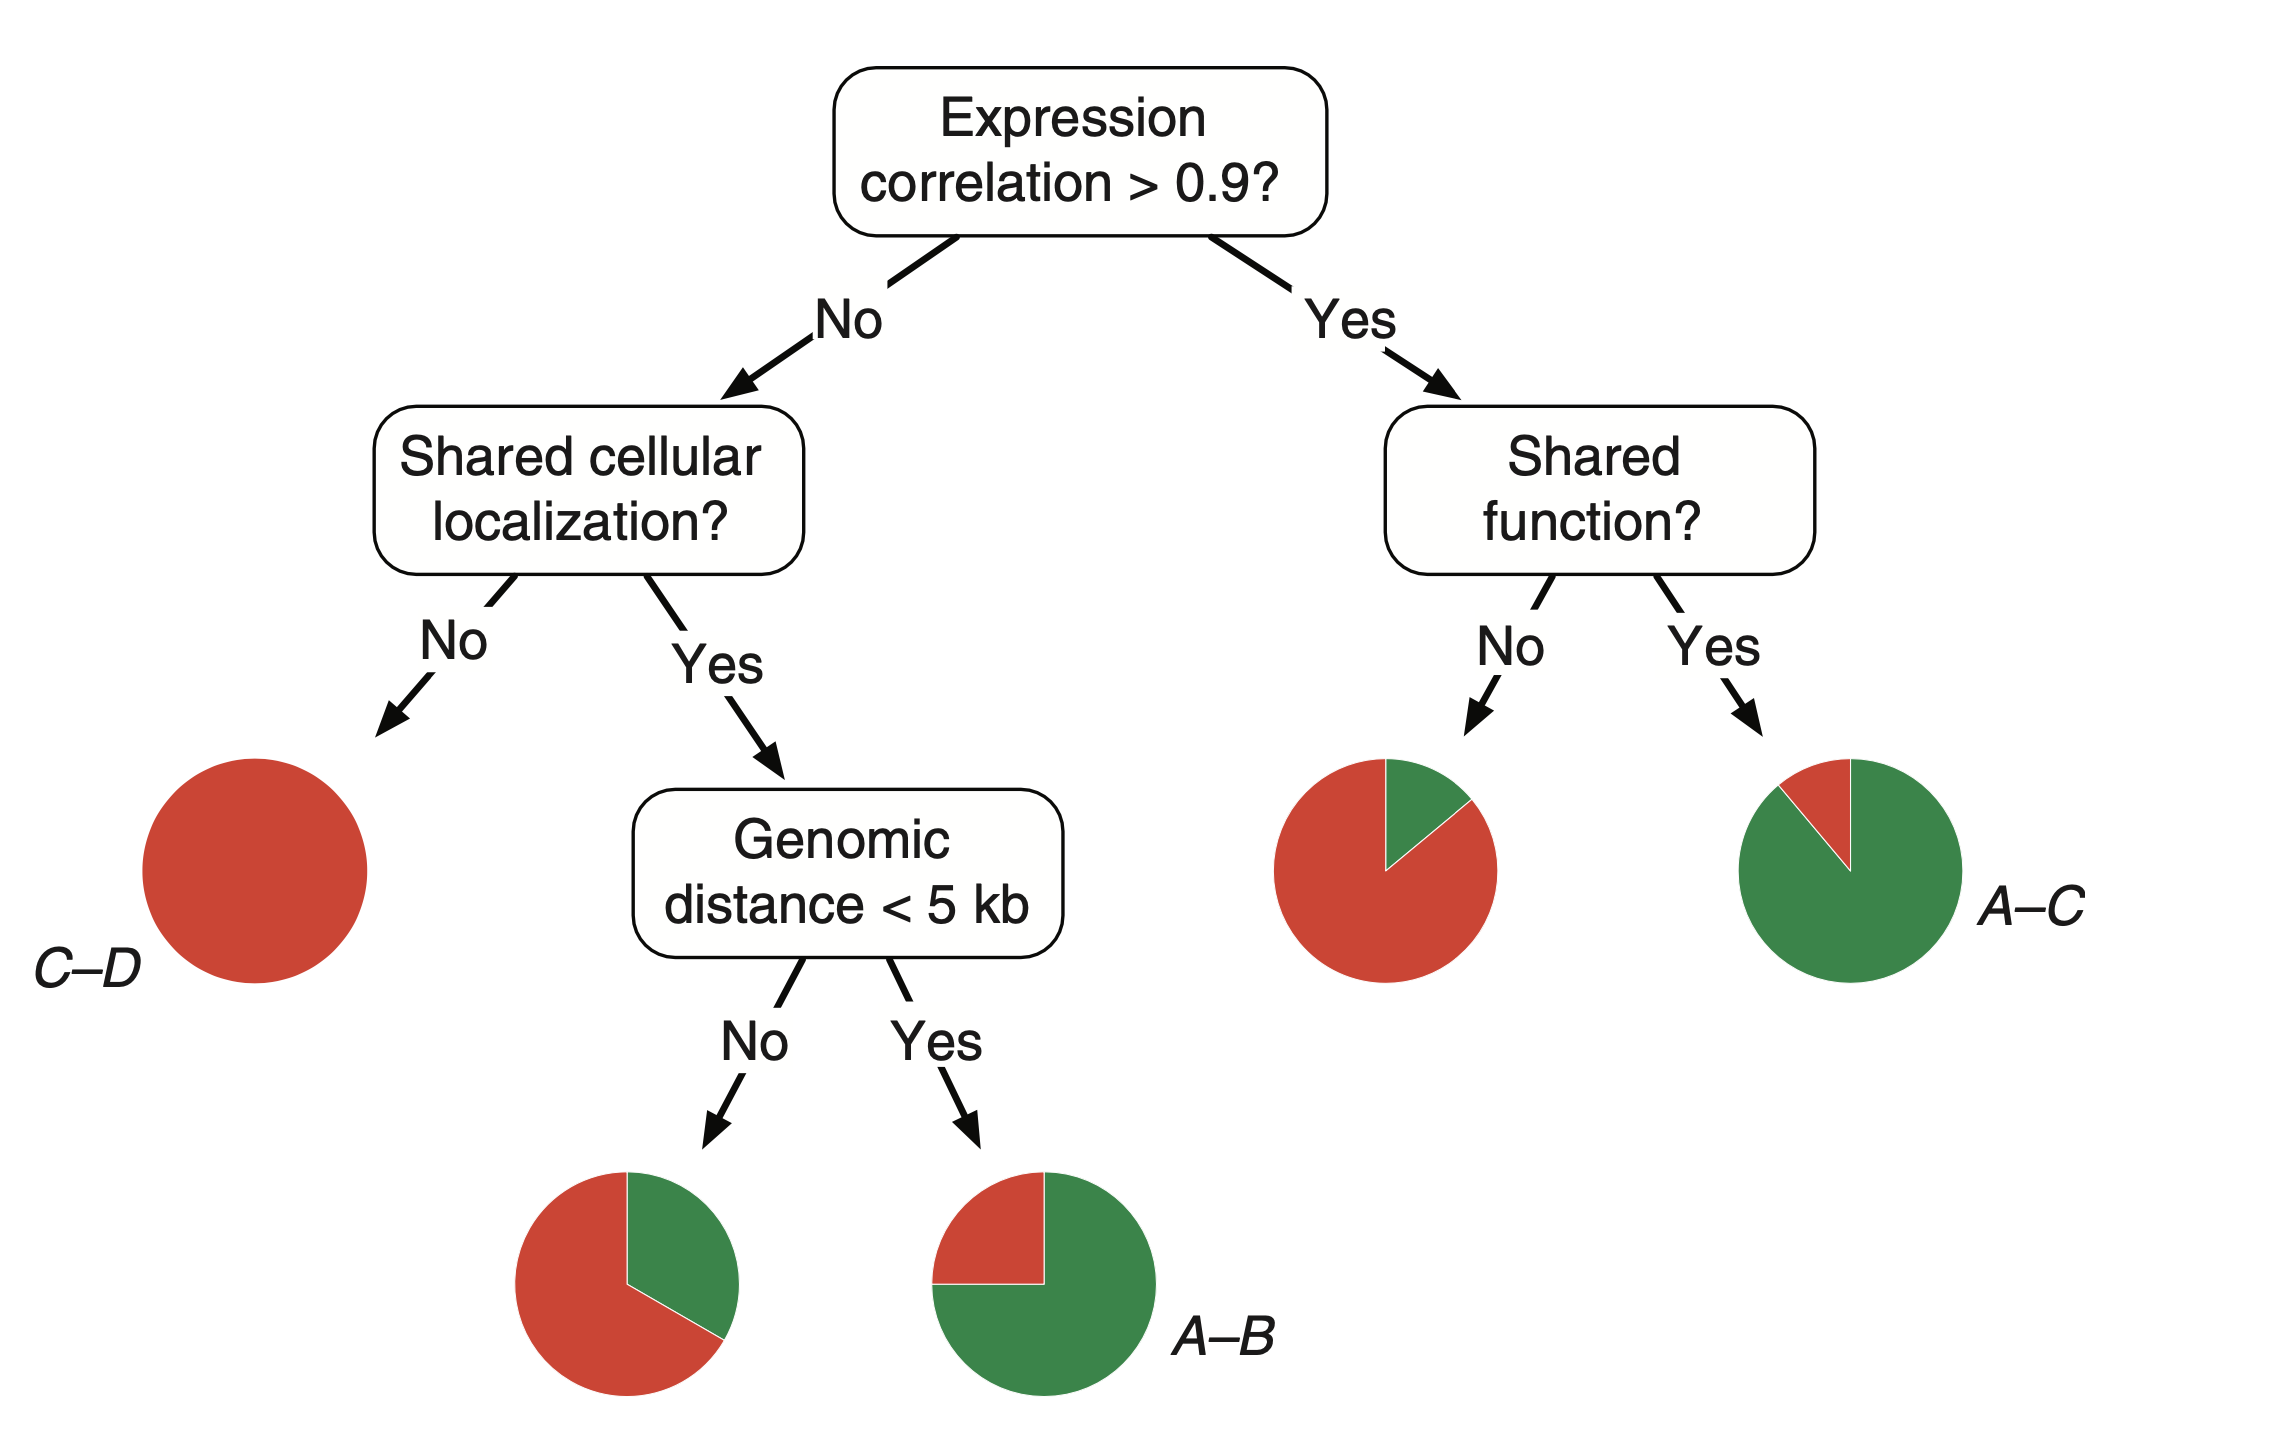
\includegraphics[width=\textwidth,height=10cm,keepaspectratio=true]{img/albero_di_decisione.png}
    \caption{
        L'immagine mostra un esempio di albero di decisione di Carl Kingsford e Steven L Salzberg ~\cite{kingsfordWhatAreDecision2008}
    }
    \label{fig:decision_tree}
\end{figure}



L'algoritmo più conosciuto che utilizza alberi di decisione è il C4.5 ~\cite{salzbergC4ProgramsMachine1994}.


\section{Dataset}

I dataset sono un insieme di dati utilizzati per l'addestramento e il test dei modelli di ML. In questa tesi sono stati utilizzati due dataset: ADFA-NET, CIDDS-18.

\subsection{ADFA-NET}

ADFA è un dataset creato da un gruppo di ricerca dell'Università di New South Wales (Australia) nel 2013 e include dieci tipi di attacchi. Contiene in particolare attacchi di Brute Force, Java Based Meterpreter, Add new Superuser, Linux Meterpreter payload e attacchi alla C100 Webshell. ~\cite{sharafaldinGeneratingNewIntrusion2018}

Questo è il più semplice dataset su cui sono stati effettuati i test.

\subsection{CIDDS-18}

Solitamente i dataset non rappresentano al meglio la realtà, in quanto per motivi di privacy questi vengono offuscati e anonimizzati perdendo molta della diversificazione utile per l'addestramento di un modello.
Per sopperire a queste mancanze è stato creato CIC-IDS cercando di mantenere il più possibile caratteristiche di uno scenario reale.
Esso contiene una grande quantità di dati ricoprendo le principali tipologie di attacchi che si possono trovare in una rete, tra questi abbiamo DoS, DDoS, Brute Force, XSS, SQL Injection, Infiltrazione, Port scan e Botnet ~\cite{sharafaldinGeneratingNewIntrusion2018}.

Questo risulta di gran lunga il più complesso dataset utilizzato in questa tesi contenendo più di settanta colonne e quasi duecentomila righe.

